% Generated from: Zhihu/专栏：概率与统计/渐近统计 (1) ：随机收敛_金鱼马_2026-04-29.md
为什么要学渐近统计？在很多时候，在固定样本，或者说非渐近 (non-asymptotic) 下，找到一个统计量的具体分布，或者进行精确的分析，往往是非常困难的。有可能是因为统计量的分布非常复杂、难以解析求解，也可能是我们的统计模型与真实分布之间存在偏差。

这时，让样本量 $n\to\infty$ 可以使问题得到简化，通常能得到对统计量分布的非常好的近似，并得到一个非常简洁的渐近分布（如正态分布）。渐近近似有很多用途：我们可将之用于渐近推断，如寻找近似的置信域和检验；也可用于从理论上研究统计推断方法的优劣，如有效性 (efficiency)。

我们首先介绍随机变量的收敛。

\begin{definition*}[随机变量、随机向量与分布函数]
对于给定的概率空间 $(\Omega,\mathscr F,P)$，（实值）随机变量定义为
$(\Omega,\mathscr F,P)\to(\mathbb R,\mathscr B_{\mathbb R})$ 的 Borel 可测映射；
$k$ 维随机向量是
\[
X=(X_1,X_2,\dots,X_k):
(\Omega,\mathscr F,P)\to(\mathbb R^k,\mathscr B_{\mathbb R^k})
\]
的 Borel 可测映射。随机向量 $X$ 的分布函数 (CDF) 定义为
\[
F_X(x):=P(X\le x)
=P(X_1\le x_1,X_2\le x_2,\dots,X_k\le x_k).
\]
\end{definition*}

\section{收敛模式}

常见的随机变量的收敛有以下三种：
\begin{definition}
设 $\{X_n\}$ 为一列 $\mathbb{R}^k$ 上的随机向量，\[ d(x, y):=\|x-y\|=\left(\sum_{i=1}^k(x_i-y_i)^2\right)^{1/2} \]为 $\mathbb{R}^k$ 中的欧式距离，诸 $\{X_n\}, X$ 定义在同一个概率空间上，
\begin{itemize}
\tightlist
\item
  \textbf{\emph{几乎必然收敛}} ：如果 $d(X_n, X) \to 0$ 的概率为1：$P(\lim_{n} d(X_n, X) = 0) = 1$ ，那么称 $\{X_n\}$ 几乎必然 (almost surely) 收敛到 $X$，我们记作 $X_n \overset{\text{a.s.}}\to X$ 。

\begin{itemize}
  \tightlist
  \item
    —— 可理解为``100\% 确信 + 100\% 精确''。
  \end{itemize}
\item
  \textbf{依概率收敛} ：如果对任意 $\epsilon > 0$，都有 $\lim\limits_{n\to\infty} P(d(X_n, X) < \epsilon) = 1$，那么称 $\{X_n\}$ 依概率收敛到 $X$，记作 $X_n \overset{P}\to X$ 。

\begin{itemize}
  \tightlist
  \item
    —— 可理解为``100\% 确信 + 不100\% 精确''。
  \end{itemize}
\item
  \textbf{$r$ \emph{阶矩收敛}} ：如果 $\lim\limits_{n\to\infty} \mathbb E[(d(X_n, X))^r ]= 0$ ，那么称 $\{X_n\}$ 按 $r$ 阶矩收敛到 $X$ ，记作 $X_n\overset{L^r}\to X$ 。
\end{itemize}
\end{definition}

在渐近分析中，最常用的收敛是依分布收敛。相比于前面的三种收敛，依分布收敛不要求 $\{X_n\}, X$ 必须在同一个概率空间中定义，因为这种收敛只关心``分布''这一统计特征。

\begin{definition}
记随机向量 $X_n$ 的分布函数为 $F_n$ 、 $X$ 的分布函数为 $F$ ，如果在 $F$ 的所有连续点 $x$ 处都有\[\lim_{n\to \infty} F_n(x) = F(x)\]
则称 $X_n$ \textbf{\emph{依分布收敛 }}到 $X$ ，记作 $X_n\overset{\rm d}\to X$ 。依分布收敛也称作弱收敛 (weak convergence) 或者 convergence in law。也有的文献记作 $X_n\rightsquigarrow X$ 。
\end{definition}

\begin{remark}

\begin{itemize}
\tightlist
\item
  分布函数总是单调非降的，因此，根据 \href{https://en.wikipedia.org/wiki/Discontinuities_of_monotone_functions}{Froda 定理}， $F$ 不连续的点至多只有可数个。
\item
  如果 $X$ 有某种特殊分布，如标准正态分布 $\mathcal N(0,1)$ ，我们也可以记作 $X_n\overset{\rm d}\to\mathcal{N}(0,1)$ 。
\end{itemize}
\end{remark}

统计学中的``渐近分布''和``渐近正态''的概念就是建立在依分布收敛上的。其定义如下：

\begin{definition}\label{def:ch1:limit-distribution}
若一列 (一维) 随机变量 $\{X_n\}$ 满足：存在常数数列 $a_n$ 以及 $b_n>0$ 和某个 (非退化) 分布 $F$ ，使得 $\frac{X_n-a_n}{b_n}\overset{\rm d}\to F$
就称 $\{X_n\}$ 有\textbf{\emph{渐近分布}} (asymptotic distribution) $F$ 。特别地，当 $F$ 是标准正态分布 $\mathcal N(0,1)$ 时，称 $\{X_n\}$ 是\textbf{\emph{渐近正态}} (asymptotically normal) 的，形式上记作 $X_n\sim A\mathcal{N}(a_n,b_n^2)$ ，这里 $a_n$ 和 $b_n$ 可以视作其渐近意义上的均值和标准差--注意，只是渐近意义上的，例如， $X_n$ 本身的均值和方差不一定存在。

这个定义可以推广到高维：设 $\{X_n\}$ 是一列 $k$ 维随机向量，如果存在一列向量 $A_n\in \mathbb R^k$ 和正定矩阵 $B_n\in\mathbb R^{k\times k}$ ，以及一个 $k$ 维分布，使得 $B_n^{-1}(X_n-A_n)\overset{\rm d}\to F$
则称 $\{X_n\}$ 有渐近分布 $F$ ；当 $F$ 是 $k$ 维标准正态分布 $\mathcal N(\bm 0,\mathbf{I}_k)$ 时，称 $X_n$ 是渐近正态的。
\end{definition}

最后，值得一提的是，依概率收敛和依分布收敛都可以视作某种度量下的收敛。

\begin{itemize}
\tightlist
\item
  定义两个随机变量 $X,Y$ 的 \emph{Ky Fan 度量}为
  \[
  d_{\text{KF}}(X,Y):=\inf\big\{\epsilon>0:P(d(X,Y)>\epsilon)\le\epsilon\big\}.
  \]
  则 $X_n\overset P\to Y$ 当且仅当 $d_{\text{KF}}(X_n,Y)\to 0$。它与某些其它的度量等价，如 $d(X,Y)=\mathbb{E}[|X-Y|\wedge 1]$ 或者 $\mathbb{E}\left[\frac{|X-Y|}{1+|X-Y|}\right]$ 。%可见 \url{https://www.zhihu.com/question/666217506/answer/1919169708051116292}。
\item
  定义两个 (一维) 分布函数 $F,G:\mathbb R\to[0,1]$ 的 \emph{Lévy 度量 }为\[ d_{\rm L}(F,G):=\inf\big\{\epsilon >0:F(x-\epsilon )-\epsilon \leq G(x)\leq F(x+\epsilon )+\epsilon ,\;\forall x\in \mathbb {R}\big\} \]那么 $X_n\overset{\rm d}\to X$ 当且仅当 $d_{\rm L}(F_n,F)\to 0$ ，其中 $F_n,F$ 分别是 $X_n$ 和 $X$ 的分布函数。%参考 \url{https://math.stackexchange.com/questions/1774319/relationship-to-weak-toplogy-l\%c3\%a9vy-metric} 和 \href{https://en.wikipedia.org/wiki/L\%C3\%A9vy\%E2\%80\%93Prokhorov_metric}{Lévy--Prokhorov metric - Wikipedia}。
\end{itemize}

\section{弱收敛的刻画}

本节来介绍一下``依分布收敛''或者说``弱收敛''能蕴含哪些结论。
先补充一下测度角度``弱极限''的概念：
\begin{definition}\label{def:ch1:weak-convergence}
设有 Polish 空间 $\mathscr X$ 和上面的 Borel $\sigma$ -代数 $\mathscr B_x$ ， $P_n,P$ 是其上的(有限) 测度，如果对任意的有界连续函数 $f:\mathscr X\to \mathbb R$ 都有
\[
\int_{\mathscr X}f(x)\mathrm dP_n(x)\to \int_{\mathscr X}f(x)\mathrm dP(x),
\]
则称测度列 $\{P_n\}$ \emph{弱收敛}到 $P$ 。
\end{definition}
不难证明，如果测度的弱极限存在，则它是唯一的。下面的 \hyperref[thm:ch1:portmanteau]{Portmanteau 定理} 告诉我们，随机变量的依分布收敛就是它们诱导出的 $\mathbb R^k$ 上测度的弱收敛。

\subsection{Portmanteau 定理}

\textbf{\emph{Portmanteau 定理 }}最初由 A. D. Alexandroff 在 1941 年给出。``Portmanteau''一词指的是一种大型旅行包，意指此定理将几种不同但完全等价的依分布收敛的方式打包在一起；它为我们提供了一个工具箱：在证明依分布收敛时，只需证明其中之一。

\begin{theorem}[Portmanteau 定理]\label{thm:ch1:portmanteau}

\label{thm:ch1:1-1}

对任意 $k$ 维随机向量 $X_n$ 和 $X$，以下陈述等价。

\begin{enumerate}
\def\labelenumi{\arabic{enumi}.}
\tightlist
\item
  依分布收敛： $X_n \overset{\rm d}\to X$；
\item
  对所有有界连续函数 $f$，有 $\mathbb{E}[f(X_n)] \to \mathbb{E}[f(X)]$；
\item
  对所有有界 Lipschitz 函数 $f$ ，有 $\mathbb{E}[f(X_n)] \to \mathbb{E}[f(X)]$；
\item
  对所有非负连续函数 $f$，有 $\liminf\limits_{n\to\infty} \mathbb{E}[f(X_n)] \geq \mathbb{E}[f(X) ]$；
\item
  对任意开集 $G$，有 $\liminf\limits_{n\to\infty} P(X_n \in G) \geq P(X \in G)$；
\item
  对任意闭集 $F$，有 $\limsup\limits_{n\to\infty} P(X_n \in F) \leq P(X \in F)$；
\item
  对任意满足 $P(X \in \partial B) = 0$ 的 Borel 集 $B$，我们称之为\emph{连续集} (continuity set)，有 $P(X_n \in B) \to P(X \in B)$。这里 $\partial B:=\overline B\setminus B^\circ$ 代表 $B$ 的\emph{边界} (boundary)。
\end{enumerate}

\end{theorem}

\begin{proof}

我们的证明顺序如图~\ref{fig:ch1:portmanteau-proof-map} 所示：

\begin{figure}[htbp]
  \centering
  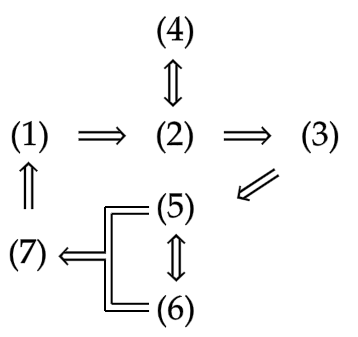
\includegraphics[width=0.4\textwidth]{figures/portmanteau-proof-map.png}
  \caption{Portmanteau 定理各条件之间的证明关系（Mathcha 绘制）}
  \label{fig:ch1:portmanteau-proof-map}
\end{figure}
\begin{itemize}[leftmargin=3cm]
  \item[(1.) $\Rightarrow$ (2.)] 不失一般性，可以设 $\sup_{x\in\mathbb R}|f(x)|\le 1$ 。先证明 $X$ 的分布函数 $F$ 连续的情形。对任意 $\epsilon>0$ ，我们可以找到足够大但有界的闭立方体 $I$ 使得 $P(X\not\in I)<\epsilon$ 。连续函数 $f$ 在紧集 $I$ 上是一致连续的，我们可以将 $I$ 划分成若干小立方体 $I=\bigcup_{j=1}^NI_j$ ，使得 $f$ 在每个 $I_j$ 上取值的差距都不超过 $\epsilon$ 。从每个 $I_j$ 中取一点 $x_j$ ，定义
  \[
  f_\epsilon(x):=\sum_{j=1}^Nf(x_j)\mathbb{I}(x\in I_j).
  \]

那么在 $I$ 上总有 $|f-f_\epsilon|<\epsilon$ 。由此得知，\[\begin{aligned} |\mathbb{E}[f(X)]-\mathbb{E}[f_\epsilon (X)]|&\le\mathbb{E}\big[|f(X)-f_\epsilon(X)|\mathbb{I}(X\in I)\big]+\mathbb{E}\big[|f(X)|\mathbb{I}(X\not\in I)\big]\\ &\le \epsilon+P(X\not\in I)\qquad {\scriptstyle |f(x)|\le 1}\\ &\le 2\epsilon \end{aligned}\]
类似地，
\[
|\mathbb{E}[f(X_n)]-\mathbb{E}[f_\epsilon (X_n)]|\le \epsilon+P(X_n\not\in I).
\]

由 $X_n\overset{\rm d}\to X$ 知有 $\lim\limits_{n\to\infty}P(X_n\not\in I)=P(X\not\in I)\le\epsilon$，因此当 $n$ 足够大时， $P(X_n\not\in I)$ 也会不超过 $\epsilon$ ，于是上式也不超过 $2\epsilon$ 。

最后，
\[
|\mathbb{E}[f_\epsilon(X_n)]-\mathbb{E}[f_\epsilon(X)]|\le \sum_{j=1}^N|P(X_n\in I_j)-P(X\in I_j)||f(x_j)|\to 0.
\]

取 $n$ 充分大使得上式不超过 $\epsilon$ 。因此，对于足够大的 $n$ ，由三角不等式，\[\begin{aligned} &|\mathbb{E}[f(X_n)]-\mathbb{E}[f(X)]|\\ \le\, &\underbrace{|\mathbb{E}[f(X_n)]-\mathbb{E}[f_\epsilon(X_n)]|}_{\le 2\epsilon}+\underbrace{|\mathbb{E}[f_\epsilon(X_n)]-\mathbb{E}[f_\epsilon(X)]|}_{\le \epsilon} + \underbrace{|\mathbb{E}[f_\epsilon(X)]-\mathbb{E}[f(X)]|}_{\le 2\epsilon}\\ \le\,& 5\epsilon \end{aligned}\]
这便证明了 (2.) 的结论。

如果 $F$ 不是连续的，我们可以沿用前面相同的证明，唯一的不同之处在于，在选择 $I_j$ （和 $I$ ）时需要让它的顶点都处于连续点（这等价于 $P(X\in \partial I_j)=0$），这样才能保证 $P(X_n\in I_j)\to P(X\in I_j)$ 。由于 $F$ 单调，不连续点至多有可数多个，换言之，其连续点集是稠密的，因此这总是做得到的。

\item[(2.) $\Rightarrow$ (3.)] 显然，因为 Lipschitz 函数一定连续。
\item[(2.) $\Leftrightarrow$ (4.) ] 先证 (2.) $\Rightarrow$(4.)，设 $f$ 非负连续，考虑截断的方法：任取 $M>0$ ，则 $f(x)\wedge M$ 是有界的，有 \[ \liminf_{n\to\infty}\mathbb{E}[f(X_n)]\ge \liminf_{n\to\infty}\mathbb{E}[f(X_n)\wedge M]\overset{\text(2.)}{=}\mathbb{E}[f(X)\wedge M] \]取 $M\to\infty$ ，由单调收敛定理，上式右侧趋于 $\mathbb{E}[f(X)]$ 。
反过来 (4.) $\Rightarrow$ (2.) ，对于任意有界连续函数 $f$ ，存在 $M$ 使得 $|f(x)|\le M$ 对任意 $x$ 成立，我们对 $g_1(x)=f(x)+M$ 和 $g_2(x)=M-f(x)$ 分别应用 (4.) 即证得 (2.)。

\item[(3.) $\Rightarrow$ (5.)] 对于任意开集 $G$ ，考虑一列 Lipschitz 函数 $f_n$ 单调递增逼近集合 $G$ 的指示函数 $\mathbb{I}_G$。例如，可以取
\[
f_m(x) = (m \cdot d(x, G^c)) \wedge 1,
\]
其中 $d(x,G^c)$ 代表点 $x$ 到闭集 $G^c$ 的距离；由于距离函数 $d(x,G^c)$ 总是 Lipschitz 的， $f_m$ 亦然；且当 $m\to\infty$ 时 $f_m\uparrow \mathbb I_G$ 。对每个固定的 $m$ ，由 (3.) 知 $\mathbb{E}[f_m(X_n)] \to \mathbb{E}[f_m(X)]$ ，从而 \[ \liminf_{n \to \infty} P(X_n \in G) \ge \liminf_{n \to \infty} \mathbb{E}[f_m(X_n)] = \mathbb{E}[f_m(X)] \]再令 $m\to\infty$ ，由单调收敛定理，上式右侧趋于 $\mathbb{E}[\mathbb I_G(X)] = P(X \in G)$ 。

\item[(5.) $\Leftrightarrow$ (6.)] 取下补集就行。
\item[(5.)+(6.) $\Rightarrow$ (7.) ] 由 (5.)、(6.)，对 Borel 集 $B$ 有
\[
P(X\in B^\circ)\le\liminf_{n\to\infty}P(X_n\in B^\circ)\le \limsup P(X_n\in \overline B)\le P(X\in\overline B).
\]
但由于 $0=P(X\in\partial B)=P(X\in\overline B)-P(X\in B^\circ)$ ，因此上面的诸不等号均取等。而 $P(X\in B)$ 和 $\lim\limits_{n\to\infty}P(X_n\in B)$ 都是上述不等式链``中间''的值，从而也相等。

\item[(7.) $\Rightarrow$ (1.)] 对任意 $F$ 的连续点 $x$ ，取 $B=(-\infty ,x]$ 。
\end{itemize}

\end{proof}

\begin{remark}

% \begin{itemize}
% \tightlist

  还有两个引申出来的等价结论：
  \begin{enumerate}
% \def\labelenumi{\arabic{enumi}.}
\tightlist
\item[8.] 对于任意有上界的上半连续函数 $f$ ，有 $\limsup\limits_{n\to\infty}\mathbb{E}[f(X_n)]\le\mathbb{E}[f(X)]$ ；
    \item[9.] 对于任意有下界的下半连续函数 $f$ ，有 $\liminf\limits_{n\to\infty}\mathbb{E}[f(X_n)]\ge\mathbb{E}[f(X)]$ 。

  \end{enumerate}

% \begin{itemize}
%   \tightlist
%   \item
    二者显然相互等价 (用 $-f$ 替代 $f$ 即可) ，我们只证明 (9.) 与定理~\ref{thm:ch1:1-1} 中诸条件的等价性。一方面 (9.) 蕴含 (4.) 是显然的；另一方面，对于下半连续函数 $f$ 和任意的 $y$ ， $\{x:f(x)>y\}$ 总是开集，由 \href{https://en.wikipedia.org/wiki/Fatou\%27s_lemma}{Fatou 引理}和 (5.)，
    \[    \liminf_{n\to\infty}\mathbb{E}[f(X_n)]=\liminf_{n\to\infty}\int_{-\infty}^\infty P(f(X_n)>y)\mathrm dy\ge \int_{-\infty}^\infty \liminf_{n\to\infty} P(f(X_n)>y)\mathrm dy\ge \int_{-\infty}^\infty P(f(X)>y)\mathrm dy=\mathbb{E}[f(X)].
    \]    从而表明了 (5.) $\Rightarrow$(9.)。
%   \end{itemize}
% \end{itemize}
\end{remark}

\subsection{渐近一致可积}

根据 Portmanteau 定理，如果 $X_n\overset{\rm d}\to X$ ，那么对任意有界连续函数 $f$ ， $\mathbb{E}[f(X_n)]\to \mathbb{E}[f(X)]$ 。有界连续这一条件是必要的，对无界的 $f$ 很容易举出来反例。特别地，对于我们同样关心的矩收敛问题，就算 $X_n\overset{\rm d}\to X$ 、或者 $X_n\overset{P}\to X$ ，也无法说明 $\mathbb{E}[X_n]\to \mathbb{E}[X]$ 或者 $\mathbb{E}[X_n^r]\to\mathbb{E}[X^r]$ 。最简单的反例是 $X_n$ 以 $\tfrac1n$ 概率取 $n^2$ 、以 $1-\tfrac1n$ 概率取 0，它依概率收敛到 0，但期望 $\mathbb{E}[X_n]=n\to\infty$ 。

连接依分布收敛和矩收敛之间缺失的环节叫做``一致可积性 (u.i.)''，

\begin{definition*}[渐近一致可积]

随机变量序列 $\{Y_n\}_{n\ge0}$ 如果满足
\[\lim_{M\to\infty}\limsup_{n\to\infty}\mathbb{E}\bigl[|Y_n|\mathbb{I}(|Y_n|>M)\bigr]=0\]
则称其为\textbf{\emph{渐近一致可积}} (asymptotically uniformly integrable) 的。

\end{definition*}

\begin{theorem}\label{thm:ch1:moment-convergence}

\label{thm:ch1:1-2}设 $X_n,X$ 是 $k$ 维随机向量，$X_n\overset{\rm d}\to X$，且函数 $f:\mathbb R^k\to\mathbb R$ 连续。若 $\{f(X_n)\}$ 渐近一致可积，则 $\mathbb{E}[f(X_n)]\to\mathbb{E}[f(X)]$。

\end{theorem}

\begin{proof}

设 $Y_n=f(X_n)$ 渐近一致可积。不失一般性设 $Y_n$ 非负，否则分别讨论其正部和负部。根据连续映射定理， $Y_n\overset{\rm d}\to Y:=f(X)$ 。再由三角不等式，对 $M>0$ ， 
\[|\mathbb{E}[Y_n]-\mathbb{E}[Y]|\le |\mathbb{E}[Y_n]-\mathbb{E}[Y_n \wedge M]|+|\mathbb{E}[Y_n\wedge M]-\mathbb{E}[Y\wedge M]|+|\mathbb{E}[Y\wedge M]-\mathbb{E}[Y]|\]
\begin{itemize}
\tightlist
\item
  首先看右式中间项，由于 $y\mapsto y\wedge M$ 连续有界，由 Portmanteau 引理之 (2.)，这一项收敛到 0；
\item
  其次看右式第一项，这一项不超过 $\mathbb{E}[Y_n\mathbb I(Y_n>M)]$ ，而由渐近一致可积条件，随着 $n\to\infty$ 并且 $M\to\infty$ ，这一项也是趋于 0 的；
\item
  最后看第三项，这一项不超过 $\mathbb{E}[Y\mathbb I(Y>M)]$ 。函数 $y\mapsto y\mathbb I(y>M)$ 下半连续，由 Portmanteau 定理的 (9.)，$\liminf\limits_{n\to\infty}\mathbb{E}[Y_n\mathbb{I}(Y_n>M)]\ge \mathbb{E}[Y\mathbb{I}(Y>M)]$，从而第三项被第一项的下极限控制；再令 $M\to\infty$，这一项也趋于 0。
\end{itemize}

\end{proof}

\begin{corollary}\label{cor:ch1:absolute-moment-convergence}

\label{cor:ch1:1-3}设 $X_n,X$ 是随机变量，$X_n\overset{\rm d}\to X$。若存在 $p>0$ 使得 $\sup_n\mathbb{E}[|X_n|^p]<\infty$，那么对所有 $0<k<p$，有绝对矩收敛 $\mathbb{E}[|X_n|^k]\to\mathbb{E}[|X|^k]$。

\end{corollary}

\begin{proof}

注意到，

\begin{equation}
\label{eq:ch1:5}
\begin{aligned} \mathbb{E}\big[|X_n|^k\mathbb I\big(|X_n|^k>M\big)\big]&\le \mathbb{E}\left[|X_n|^k\left(\frac{|X_n|^k}{M}\right)^{(p-k)/k}\mathbb I\big(|X_n|>M^{1/k}\big)\right]\\ &=M^{1-p/k}\mathbb{E}\Big[|X_n|^p\mathbb I\big(|X_n|>M^{1/k}\big)\Big]\\ &\le M^{1-p/k}\mathbb{E} [|X_n|^p]\end{aligned}
\end{equation}

当 $k<p$ 时 $M$ 的指数是负数，且 $\sup_n\mathbb{E}[|X_n|^p]<\infty$，所以式~\eqref{eq:ch1:5} 的右端关于 $n$ 一致地趋于 0。故 $|X_n|^k$ 渐近一致可积，由定理~\ref{thm:ch1:1-2} 即得结论。

\end{proof}

\subsection{连续映射定理}

\textbf{\emph{连续映射定理}} (Continuous mapping theorem) 回答的是这样的问题：若 $\{X_n\}$ 以某种方式收敛到 $X$ ，那么，在一个连续变换 $g$ 下，这种收敛能否保持？答案是肯定的，

\begin{theorem}[连续映射定理]\label{thm:ch1:continuous-mapping}

\label{thm:ch1:1-4}

设 $\{X_n\}$ 和 $X$ 是 $k$ 维随机变量，$g:\mathbb R^k\to\mathbb R^m$ 在某集合 $C$ 上处处连续，且 $P(X\in C)=1$。那么

\begin{enumerate}
\def\labelenumi{\arabic{enumi}.}
\tightlist
\item
  若 $X_n\overset{\rm d}\to X$ ，则 $g(X_n)\overset{\rm d}\to g(X)$ ；
\item
  若 $X_n \overset{P}\to X$，则 $g(X_n) \overset{P}\to g(X)$；
\item
  若 $X_n \overset{\text{a.s.}}\to X$，则 $g(X_n) \overset{\text{a.s.}}\to g(X)$。
\end{enumerate}

\end{theorem}

\begin{proof}
\begin{enumerate}
  \item[(1.)] 考虑利用 Portmanteau 定理（定理~\ref{thm:ch1:1-1}）的第 (6.) 项。对任意闭集 $F\subset \mathbb R^m$ ，我们首先表明：
\[\overline{g^{-1}(F)}\subset g^{-1}(F)\cup C^c\]
上面第二个包含关系之所以成立，是因为：对任意 $x\in\overline{g^{-1}(F)}$ ，存在一列 $\{x_j\}\subset g^{-1}(F)$ 使得 $x_j\to x$ ，这样一来：如果 $x\in C$ ，那么由连续性知 $g(x_j)\to g(x)$ ，由诸 $g(x_j)\in F$ 且 $F$ 闭，知 $g(x)\in F$ ；否则 $x\in C^c$ ；无论如何，总有 $x\in g^{-1}(F)\cup C^c$ 。

那么我们直接证明
\[\begin{aligned} \limsup_{n\to\infty} P(g(X_n) \in F) &\le \limsup_{n\to\infty} P(X_n \in \overline{g^{-1}(F)})\qquad \text{\scriptsize 由}{\scriptstyle g^{-1}(F)\subset \overline{g^{-1}(F)}}  \\ &\le P(X \in \overline{g^{-1}(F)}) \qquad \text{\scriptsize 由 Portmanteau 定理 (6.)} \\ &\le P(X \in g^{-1}(F)) + \underbrace{P(X \notin C) }_{=0}\qquad \text{\scriptsize 由 (}{\scriptstyle *}\text{\scriptsize ) 式} \\ &= P(g(X) \in F) \end{aligned}\]
从而由 Portmanteau 定理， $g(X_n)\overset{\rm d}\to g(X)$ 。

\item[(2.)] 任取 $\epsilon>0$ ，考虑这样的一个集合：它包含了那些``附近存在 $g$ 的跳跃超过 $\epsilon$ 的点''：
\[
B_\delta = \big\{ x \in\mathbb R^k: \text{ 存在 } y \text{ 使得 } |x - y| < \delta \text{ 但 } |g(x) - g(y)| > \epsilon \big\}.
\]

于是
\[
P(|g(X_n)-g(X)|>\epsilon)\le P(X\in B_\delta)+P(|X_n-X|\ge\delta).
\]

观察上式：

\begin{itemize}
\tightlist
\item
  对右侧第一项 $P(X\in B_\delta)$，由 $P(X\in C)=1$ 有 $P(X\in B_\delta)=P(X\in B_\delta\cap C)$。当 $\delta\downarrow 0$ 时，$B_\delta\cap C\downarrow\varnothing$，故概率的上连续性给出 $P(X\in B_\delta)\to 0$；
\item
  由依概率收敛的定义，第二项 $P(|X_n-X|>\delta)$ 在 $n\to\infty$ 时也收敛于 0。
\end{itemize}

从而 $P(|g(X_n)-g(X)|>\epsilon)\to 0$ ，即 $g(X_n)\overset P\to g(X)$ 。

\item[(3.)] 其实是显然的，直接由连续性得到。
\end{enumerate}


\end{proof}

连续映射定理看起来表述很简单，但却非常实用。我们举几个简单的小例子。

\begin{example}[连续映射定理的简单应用]

\begin{itemize}
\tightlist
\item
  如果 $X_n \overset{\rm d}\to X \sim\mathcal N(0, 1)$，那么 $X_n^2 \overset{\rm d}\to \chi_1^2$。
\item
  如果 
  \[  \begin{pmatrix} X_n \\ Y_n \end{pmatrix} \overset{\rm d}\to \mathcal N_2\left(\begin{pmatrix} 0 \\ 0 \end{pmatrix}, \begin{pmatrix} 1 &0\\ 0&1 \end{pmatrix}\right)
  \]  那么 $X_n / Y_n$ 依分布收敛于 Cauchy 分布。%，见\href{https://www.zhihu.com/question/29552486/answer/44756825}{两个独立正态分布的随机变量的比值，服从怎样的分布？}。
\item
  设 $X_1,X_2,\dots,X_n$ 是来自某总体的 i.i.d. 样本，记总体均值为 $\mu$ 、总体二阶原点矩为 $\mu_2<\infty$ 、总体方差为 $\sigma^2<\infty$ ，样本方差为 $S_n^2 = \frac{1}{n-1}\sum (X_i - \bar{X})^2$。令 $Y_i = (X_i, X_i^2)^\top$。由强大数律， 
  \[  \frac{1}{n}\sum_{i=1}^{n} Y_i = \begin{pmatrix} \frac{1}{n}\sum_{i=1}^{n} X_i \\ \frac{1}{n}\sum_{i=1}^{n} X_i^2 \end{pmatrix} \overset{\text{a.s}}\to \begin{pmatrix} \mu \\ \mu_2 \end{pmatrix}
  \]  令 $g(x, y) = y - x^2$。由连续映射定理： 
  \[  S_n^2 = g\left(\bar{X}, \frac{1}{n}\sum_{i=1}^{n} X_i^2\right) \overset{\text{a.s.}}\to \mu_2 - \mu^2 = \sigma^2
  \]  再次应用连续映射定理得 $S_n \overset{\text{a.s.}}\to \sigma$。
\item
  如果 $X_n \overset{\rm d}\to \mathcal N_k(\mu, \Sigma)$ ，那么对任意常数矩阵 $C \in \mathbb{R}^{m \times k}$， 
  \[  C X_n \overset{\rm d}\to \mathcal N_m(C\mu, C\Sigma C^\top).
  \]\end{itemize}

\end{example}

\subsection{Polya 定理}

\textbf{\emph{Polya 定理 }}的结论是：依分布收敛蕴含分布函数的一致收敛。

\begin{theorem}[Pólya 定理]\label{thm:ch1:polya}

\label{thm:ch1:1-5}

设 $X_n \overset{\rm d}\to X$，$F_n$ 和 $F$ 分别是 $k$ 维随机向量 $X_n$ 和 $X$ 的分布函数，且 $F$ 连续。那么当 $n \to \infty$ 时，
\[
\sup_{x\in\mathbb R^k}|F_n(x)-F(x)|\to0.
\]

\end{theorem}

\begin{proof}

先证明一维情形。对给定的正整数 $N$ ，根据 $F$ 的连续性和单调性，我们总可以找到 $-\infty= x_0<x_1<\dots<x_N=\infty$ ，使得 $F(x_i)=\frac iN,\;i=0,1,\dots,N$ 。对于 $x_{i-1}\le x\le x_i$ ，有
\[\begin{aligned} F_n(x)-F(x)&\le F_n(x_{i})-F(x_{i-1})=F_n(x_{i})-F(x_{i})+\frac 1N\\ F_n(x)-F(x)&\ge F_n(x_{i-1})-F(x_{i})=F_n(x_{i-1})-F(x_{i-1})-\frac 1N\\ \end{aligned}\]
因此，对每个 $x$ 都有 \[|F_n(x)-F(x)|\le \sup_{i=0,1,\dots,N}|F_n(x_i)-F(x_i)|+\frac1N.\]
当 $n\to\infty$ 时有 $F_n(x_i)\to F(x_i)$ ，故上式右侧第一项会趋于 0；再令 $N\to\infty$ ，就证明了结论。

在高维情况下，证明也是完全类似的，只需改用 $k$ 维超立方体来划分 $\mathbb R^k$ 。

\end{proof}

\section{各种收敛的关系}

\begin{theorem}\label{thm:ch1:convergence-relations}

\label{thm:ch1:1-6}

设 $X_n, X$ 和 $Y_n$ 为同一概率空间上的随机向量。则

\begin{enumerate}
\def\labelenumi{\arabic{enumi}.}
\tightlist
\item
  $X_n \overset{\text{a.s.}}\to X$ 蕴含 $X_n \overset P\to X$；
\item
  $X_n \overset P\to X$ 蕴含 $X_n \overset{\rm d}\to X$；
\item
  设 $c$ 为常向量，则 $X_n \overset P\to c$ 当且仅当 $X_n\overset{\rm d}\to c$ ；
\item
  若 $X_n\overset{\rm d}\to X$ 且 $d(X_n, Y_n)\overset P\to 0$，则 $Y_n\overset{\rm d}\to X$；
\item
  设 $c$ 为常向量，若 $X_n\overset{\rm d}\to X$ 且 $Y_n\overset P\to c$ ，则 $(X_n, Y_n)\overset{\rm d}\to (X, c)$；
\item
  若 $X_n\overset P\to X$ 且 $Y_n \overset P\to Y$，则 $(X_n, Y_n)\overset P\to (X, Y)$。
\end{enumerate}

\end{theorem}

\begin{proof}

\begin{enumerate}
  \item[(1.)] 任取 $\epsilon>0$，令 $A_n=\bigcup_{m\ge n}\{\omega:d(X_m(\omega),X(\omega))>\epsilon\}$。集合列 $\{A_n\}$ 递减，且 $\bigcap_nA_n$ 是偏差超过 $\epsilon$ 无穷多次发生的事件。若 $X_n\overset{\mathrm{a.s.}}\to X$，则 $P(\bigcap_nA_n)=0$；由概率的上连续性，$P(A_n)\to0$。于是 $P(d(X_n,X)>\epsilon)\le P(A_n)\to0$。
  \item[(4.)] 对于有界 Lipschitz 函数 $f$，设其 Lipschitz 常数为 $L$ ；任取 $\epsilon > 0$，有：
\[\begin{aligned}  |\mathbb{E} [f(X_n)] - \mathbb{E} [f(Y_n)]|     &\le \mathbb{E}\Big[\big|f(X_n) - f(Y_n)\big| \mathbb{I}\big(d(X_n, Y_n)\le \epsilon\big)\Big] + \mathbb{E}\Big[\big|f(X_n) - f(Y_n)\big| \mathbb{I}\big(d(X_n, Y_n) > \epsilon\big)\Big] \\ &\le L\epsilon \cdot P(d(X_n, Y_n) \le \epsilon) + 2 \sup_{x\in\mathbb R} |f(x)|\cdot P(d(X_n, Y_n) > \epsilon)    \end{aligned}\]
上式第二项随着 $n\to\infty$ 趋于 0，而第一项中包含 $\epsilon$ ，从而可以任意小，表明 $\mathbb E [f(Y_n)] \to \mathbb E [f(X_n)]$。由 Portmanteau 定理的 (3.) 即证 $Y_n\overset{\rm d}\to X$。

  \item[(2.)] 由 $d(X_n,X)\overset P\to 0$ 和 (4.) 直接推出。
  \item[(3.)] 必要性由 (2.) 显然，仅证充分性。设 $X_n\overset{\rm d}\to c$ ，利用 Portmanteau 定理的 (3.)，
\[\begin{aligned} \limsup_{n\to\infty} P(d(X_n,c)\ge\epsilon) \le P(d(c,c)\ge \epsilon)=0 \end{aligned}\]
从而 $P(d(X_n,c)\ge\epsilon)\to 0$ ，即 $X_n\overset P\to c$ 。
  \item[(5.)] 注意到 $d\big((X_n,Y_n),(X_n,c)\big)=d(Y_n,c)\overset P\to 0$ ，因此由 (4.)，我们只需证明 $(X_n,c)\overset{\rm d}\to (X,c)$ 。对任意有界连续函数 $f(x,y)$ ，固定 $y=c$ ， $x\mapsto f(x,c)$ 依然是有界连续的，由 $X_n\overset{\rm d}\to X$ 和 Portmanteau 定理的 (2.) 有 $\mathbb{E}[f(X_n,c)]\to \mathbb{E}[f(X,c)]$ 。
  \item[(6.)] 利用 $d\big((X_n,Y_n),\, (X,Y)\big) \le d(X_n,X) + d(Y_n,Y)$ 即得。

\end{enumerate}


\end{proof}

由定理~\ref{thm:ch1:1-6} 可知：

\begin{itemize}
\tightlist
\item
  (1.) (2.) 叙述了三种不同收敛模式的``强弱''：a.s. 收敛最强、依概率收敛次之，依分布收敛最弱。
\item
  (6.) 告诉我们：边际依概率收敛 $\Rightarrow$ 联合依概率收敛。反之，由连续映射定理（ $(x,y)\mapsto x$ 和 $(x,y)\mapsto y$ 都是连续的），联合依概率收敛也蕴含边际依概率收敛。因此， 边际依概率收敛\textbf{$\Leftrightarrow$} 联合依概率收敛。
    但注意在依分布收敛的情况下情形不太相同。由连续映射定理，联合依分布收敛可以推出边际依分布收敛，但是，边际依分布收敛\emph{不能}推出联合依分布收敛。这是因为联合分布不仅取决于边际分布，还取决于变量间的依赖结构 （即 ``Copula''）。
\item 
  在渐近正态的情形：若 $X_n\sim A\mathcal N(\mu,b_n^2)$ ，且其渐近方差 $b_n^2\to 0$ ，那么 $X_n\overset{\rm d}\to \mu$ 且 $X_n\overset P\to \mu$ 。
\end{itemize}

此外还有一个重要推论，即 \textbf{\emph{Slutsky 定理}}：

\begin{corollary}[Slutsky 定理]\label{cor:ch1:slutsky}

\label{cor:ch1:1-7}设 $X_n,X,Y_n$ 是随机向量， $c$ 是常量，且 $X_n\overset{\rm d}\to X$ 、 $Y_n\overset P\to c$ ，那么

\begin{enumerate}
\def\labelenumi{\arabic{enumi}.}
\tightlist
\item
  $X_n+Y_n\overset{\rm d}\to X+c$ ；
\item
  $Y_nX_n\overset{\rm d}\to cX$ ；
\item
  若 $c\ne 0$ ，则 $X_n/Y_n\overset{\rm d}\to X/c$ 。
\end{enumerate}

\end{corollary}

\begin{proof}

由定理~\ref{thm:ch1:1-6} 的 (5.)，$(X_n, Y_n)\overset{\rm d}\to (X, c)$。再对 $(x,y)\mapsto x+y,\,xy,\,x/y$ 分别应用连续映射定理即证。

\end{proof}

\begin{remark}

\begin{itemize}
\tightlist
\item
  这里第 (1.) 条要求 $X_n,X,Y_n$ 是同一维度的；在第 (2.)、(3.) 条里，我们假设 $Y_n,c$ 都是一维的。
\item
  根据定理~\ref{thm:ch1:1-6} 的 (6.)，若把 Slutsky 定理结论中的`` $\overset{\rm d}\to$ ''全部换成 $\overset P\to$ ，则结论仍成立。
\item
  Slutsky 定理实际上对随机矩阵也成立，不过要将 (3.) 改成：若 $c$ 可逆，则 $Y_n^{-1}X_n\overset{\rm d}\to c^{-1}X$ 。在回归分析，如 OLS 估计量的渐近分析时，我们便可用到随机矩阵形式的 Slutsky 定理。
\end{itemize}
\end{remark}

\begin{example}[$t$-统计量的渐近分布]
设 $Y_{1}, \ldots , Y_{n}$ i.i.d. 来自分布 $F$，有均值为 0，方差 $0<\sigma^2<\infty$。t-统计量为：$t_{n} := \sqrt{n} \bar{Y} / S_{n}$。 由于样本方差
\[\begin{aligned} S_n^2 &= \frac{1}{n - 1}\sum_{i = 1}^n(Y_i - \bar{Y})^2 \\ &= \frac{n}{n - 1}\left(\frac{1}n\sum_{i = 1}^nY_i^2 - \bar{Y}^2\right) \\ &\overset P\to  1 \cdot (\mathbb E [Y_i^2] - (\mathbb E [Y_i])^2)\\  &= \mathbb E [Y_i^2] =\sigma^2\end{aligned}\]
因此由连续映射定理， $S_{n}\overset P\to \sigma$。

另一方面，由中心极限定理，
\[\sqrt{n} \bar{Y}\overset{\rm d}\to N(0, \sigma^2)\]
因此，Slutsky 定理告诉我们
\[t_n=\frac{\sqrt{n} \bar{Y}}{S_{n}} \overset{\rm d}\to \frac{\mathcal{N}(0,\sigma^2)}{\sigma}= \mathcal{N}(0, 1)\]

\end{example}

\section{Prohorov 定理}

我们熟知数学分析里的 ``Bolzano－Weierstrass 聚点定理''： $\mathbb R^k$ 中的任意有界无限点集必存在聚点；或者更简单地，``有界序列一定存在收敛子列''。正如同数列一样，考察随机变量列的子列收敛性也是非常重要的。能否将聚点原理推广到随机变量空间的弱收敛呢？很容易举出例子，表明不满足某种``有界''性质的一列随机变量不存在``聚点''，例如 $X_1,X_2,\dots$ ，其中 $X_n \sim \mathcal N(0,n^2)$ ，那么不存在任意一个子列依分布收敛。所以，必须找到某种``有界''来限制。
\begin{definition}
  为此，我们引入``胎紧''的概念。给定一族随机向量 $\{X_\alpha:\alpha\in A\}$ ，若对任意 $\epsilon>0$ ，都存在常数 $M$ 使得 $\sup_{\alpha\in A}P(\|X_\alpha\|>M)<\epsilon$ ，则称这族随机变量是 (一致) \textbf{\emph{胎紧}} (uniformly tight) 或者\emph{随机有界} (bounded in probability) 的。
\end{definition}

\begin{remark}
胎紧有更``专业''一些的描述：给定 Polish 空间 $\Omega$ 上的一族概率测度 $\{P_\alpha:\alpha\in A\}$，若其满足：对任意 $\epsilon$，总存在紧集 $K\subset \Omega$，使得对每个 $\alpha$ 都有 $P_\alpha(K)>1-\epsilon$。本质上，``一致胎紧''表明一族分布一致地集中在一个紧集上。
\end{remark}

一个简单的例子是，单独的一个随机量 $X$ 一定是胎紧的，因为 $\lim\limits_{M\to\infty} P(\|X\|>M)=0$ 。进一步，有限个随机向量 $\{X_n\}_{n=1}^N$ 也是一致胎紧的。

在这一观察下，不难看出：一列随机向量 $\{X_n\}_{n=1}^\infty$ 是胎紧的，当且仅当：对任意 $\epsilon>0$ ，都存在常数 $M$ 和 $N$ 使得对任意 $n>N$ 有 $P(\|X_n\|>M)<\epsilon$ 。这是因为，前面有限多项 $\{X_n\}_{n=1}^{N}$ 总是胎紧的，我们总可以适当增大 $M$ ，使得整个序列胎紧。

\begin{theorem}[Prohorov 定理]\label{thm:ch1:prohorov}

\label{thm:ch1:1-8}

\begin{enumerate}
\def\labelenumi{\arabic{enumi}.}
\tightlist
\item
  如果 $X_n \overset{\rm d}\to X$，那么 $\{X_n\}_{n=1}^\infty$ 是胎紧的。
\item
  如果 $\{X_n\}_{n=1}^\infty$ 是胎紧的，那么存在一个子列 $\{X_{n_j}\}$，使得当 $j \to \infty$ 时，$X_{n_j}\overset{\rm d}\to X$。
\end{enumerate}

\end{theorem}

\begin{proof}

\begin{enumerate}
  \item[(1.)] 由于单个随机向量 $X$ 胎紧，任取 $\epsilon>0$，都可以选取 $M$ 使得 $P(\|X\|\ge M)<\epsilon$。根据 Portmanteau 定理 (6.)，$\limsup\limits_{n\to\infty}P(\|X_n\|\ge M)\le P(\|X\|\ge M)<\epsilon$。这表明存在 $N$，使得 $n\ge N$ 时都有 $P(\|X_n\|>M)<2\epsilon$，再适当增大 $M$ 以控制前 $N-1$ 项，即得整列 $\{X_n\}_{n=1}^\infty$ 胎紧。
  \item[(2.)] 证明需要用到一个引理，称作 \textbf{\emph{Helly 选择引理}} ：对任意给定的 $\mathbb R^k$ 上的分布函数列 $\{F_n\}$ ，总存在其子列 $\{F_{n_j}\}$ 和一个右连续的单调非降函数 $F:\mathbb R^k\to[0,1]$ ，使得 $F_{n_j}$ 逐点收敛到 $F$ ，即，对每个 $F$ 的连续点 $x$ 都有 $F_{n_j}(x)\to F(x),\,j\to\infty$ （注意这里 $F$ 不一定是分布函数）。
% 一个一维情形的证明可以参考（高维情形类似）：

% \href{https://zhuanlan.zhihu.com/p/1901931034704082802}{海利选择定理 (一) (Helly's Selection Theorem)}

先证明一维情形。记 $X_n$ 的分布函数为 $F_n$。根据 Helly 选择引理，存在子列 $F_{n_j}$，在某右连续单调非降函数 $F$ 的每个连续点处收敛到 $F$。由胎紧性，对任意 $\epsilon>0$，可取 $M>0$ 使得对所有 $n$ 都有 $P(|X_n|>M)<\epsilon$；还可调整 $M$，使 $M$ 和 $-M$ 都是 $F$ 的连续点。于是 $F_n(-M)\le\epsilon$ 且 $F_n(M)\ge1-\epsilon$，令 $j\to\infty$ 得 $F(-M)\le\epsilon$ 且 $F(M)\ge1-\epsilon$。再令 $M\to\infty$，可知 $F(-\infty)=0$、$F(+\infty)=1$，所以 $F$ 是某随机变量 $X$ 的分布函数。由分布函数收敛判据，$X_{n_j}\overset{\rm d}\to X$。高维情形用紧立方体 $[-M,M]^k$ 和多维 Helly 选择引理作同样论证。

\end{enumerate}

\end{proof}

\begin{remark}

  Prohorov 定理可以表述成：在 Polish 空间上，一族概率测度是胎紧的当且仅当它 (在弱收敛拓扑下) \emph{相对紧} 。所谓``相对紧''的定义为：在 Polish 空间上的测度族 $\{P_\alpha,\alpha\in\Lambda\}$ 若满足：从任意的序列 $\{P_{\alpha_n}\}$ 中都存在弱收敛子序列，那么称 $\{P_\alpha\}$ 是 (弱) 相对紧的。注意，这个定义里子列弱收敛的极限测度不一定在族 $\{P_\alpha\}$ 中。也可以说， $\{P_\alpha\}$ 的闭包在弱收敛拓扑下是紧的。
\end{remark}

这个定理在随机收敛的证明中很有用，我们在后文中将介绍的 Lévy 连续定理便是一例（见定理~\ref{thm:ch2:levy-continuity}）。

\section{随机阶}


\begin{definition}
  
设 $\{X_n\}$ 是一列随机向量，

\begin{itemize}
\tightlist
\item
  若 $X_n\overset P\to 0$ ，记为 $X_n=o_P(1)$ ；
\item
  若 $\{X_n\}$ 是随机有界 (胎紧) 的，记为 $X_n=O_P(1)$ 。
\end{itemize}


进一步，设 $\{a_n\}$ 是常数数列：

\begin{itemize}
\tightlist
\item
  若 $X_n=a_nY_n$ 且 $Y_n=o_P(1)$ ，记作 $X_n=o_P(a_n)$ ；
\item
  若 $X_n=a_nY_n$ 且 $Y_n=O_P(1)$ ，记作 $X_n=O_P(a_n)$ 。
\end{itemize}


符号 $o_P$ 和 $O_P$ 方便地描述了随机序列的行为，它们被称作\textbf{\emph{随机阶}} (Stochastic Orders)。
\end{definition}

\begin{example}[Chebyshev 不等式与随机阶]
设有一列随机变量 $\{X_n\}$ ，对任意 $n$ 有 $\mathbb{E}[X_n]=\mu_n$ 、 $\mathrm{Var}[X_n]=\sigma_n^2<\infty$ 。由 Chebyshev 不等式，
\[P\left(\sigma_n^{-1}|X_n - \mu_n| > M\right) \le  \frac{1}{M^2}\]
对任意 $\epsilon > 0$，选择 $M$ 使得 $M^{-2} < \epsilon$，则有
\[P\left(\sigma_n^{-1}|X_n - \mu_n| > M\right) < \epsilon\]
这意味着 $X_n-\mu_n=O_P(\sigma_n)$。

设 $Y_{1}, \ldots , Y_{n}$ i.i.d. 来自分布 $F$，均值为 $\mu$ 、方差为 $0<\sigma^2<\infty$ ，那么样本均值 $\bar Y=\frac1n\sum\limits_{j=1}^n Y_j$ 的期望为 $\mu$ 、方差为 $\sigma^2/n$ 。用上面的结论，可知 $\bar{Y}-\mu=O_P(n^{-1/2})$ 。


\end{example}

如果我们想找一个估计量 $T_n$ 的渐近分布，一般的方法是找到它的一个分解 $T_n=L_n+P_n$ ，以及一个适当的阶 $\{a_n\}$ 满足 $L_n=O_P(a_n)$ 且 $P_n=o_P(a_n)$ ，则 $T_n/a_n=L_n/a_n+o_P(1)$ ，根据 Slutsky 定理（推论~\ref{cor:ch1:1-7}），第二项总是可以忽略的，问题便化作分析 $L_n/a_n$ 的渐近分布。

$o_P$ 和 $O_P$ 符号遵循一些运算法则，我们常常不加说明地使用，如下：

\begin{enumerate}
\def\labelenumi{\arabic{enumi}.}
\tightlist
\item
  $o_P(1) + o_P(1) = o_P(1)$；
\item
  $O_P(1) + O_P(1) = O_P(1)$ ；
\item
  $o_P(1) + O_P(1) = O_P(1)$；
\item
  $O_P(1) \cdot o_P(1) = o_P(1)$；
\item
  $(1 + o_P(1))^{-1} = O_P(1)$；
\item
  $o_P(O_P(1)) = O_P(o_P(1)) = o_P(1)$。
\end{enumerate}

这里的等号应该视作``左侧能推出右侧''的含义。

下面是一个稍微复杂一点的规则：

\begin{lemma}[Stochastic Plug-in]\label{lem:ch1:stochastic-plugin}

\label{lem:ch1:1-9}

设 $R: \mathbb{R}^k \mapsto \mathbb{R}$ 为一实函数，且 $R(0) = 0$。 $\{X_n\}$ 为取值于 $R$ 定义域内的随机变量序列，且 $X_n\overset P\to 0$。那么对任意 $p > 0$，

\begin{enumerate}
\def\labelenumi{\arabic{enumi}.}
\tightlist
\item
  若当 $h \to 0$ 时 $R(h) = o(\|h\|^p)$，则 $R(X_n) = o_P(\|X_n\|^p)$；
\item
  若当 $h \to 0$ 时 $R(h) = O(\|h\|^p)$，则 $R(X_n) = O_P(\|X_n\|^p)$。
\end{enumerate}

\end{lemma}

\begin{proof}
\begin{enumerate}
  \item [(1.)] 由 $R(h) = o(\|h\|^p),\,h\to 0$ 知 $R$ 在 0 处连续。令
\[g(h) = \begin{cases} R(h) / \|h\|^p, & h \neq 0 \\ 0, & h=0 \end{cases}\]
则 $g$ 在 0 处连续，且 $R(X_n) = \|X_n\|^p g(X_n)$。由连续映射定理：
\[g(X_n) \overset P\to g(0) = 0\]
因此 $R(X_n) = o_p(\|X_n\|^p)$。

  \item[(2.)]  $g(h)$ 定义同前。由 $R(h) = O(\|h\|^p)$ 知 $g$ 在 $h=0$ 附近有界，即，存在 $M, \delta > 0$，使得对所有 $\|h\| < \delta$，有 $|g(h)| \le M$。因此，
\[\{\omega : |g(X_n(\omega))| > M\} \subset \{\omega : \|X_n(\omega)\| \ge \delta\}\]
于是，
\[P(|g(X_n)| > M) \le P(\|X_n\| \ge \delta) \to 0,\quad\text{ 当 } n\to\infty\]
这说明 $g(X_n) = O_p(1)$，从而 $R(X_n) = O_p(\|X_n\|^p)$。

\end{enumerate}

\end{proof}

\begin{example}[样本方差的渐近分布]
设 $X_{1},\ldots ,X_{n}$ i.i.d. 来自分布 $F$，均值为 $\mu$ 、方差为 $0<\sigma^2<\infty$ ，且 $\mathbb{E}[X_1^4]<\infty$ 。那么样本方差
\[\begin{aligned} S_{n} &= \frac{1}{n}\sum_{i = 1}^{n}(X_{i} - \bar{X})^{2} = \frac{1}{n}\sum_{i = 1}^{n}(X_{i} - \mu)^{2} - (\bar{X} - \mu)^{2} \end{aligned}\]
（除以 $n$ 或者 $n-1$ 不影响渐近结论。）

由于 $\mathbb E [X^4]< \infty$，由中心极限定理，
\[\sqrt{n}\left(\frac{1}{n}\sum_{i = 1}^{n}(X_{i} - \mu)^{2} - \sigma^{2}\right) \overset{\rm d}\to N(0,\nu^{2})\]
其中 $\nu^{2} := \text{Var}[(X_1 - \mu)^2]$。

另一方面，$\bar{X} - \mu = O_P(n^{-1/2})$，所以 $\sqrt{n} (\bar{X} - \mu)^2 = O_P(n^{-1/2}) = o_p(1)$。由 Slutsky 定理，
\[\begin{aligned} \sqrt{n}(S_{n} - \sigma^{2}) &= \sqrt{n}\left(\frac{1}{n}\sum_{i = 1}^{n}(X_{i} - \mu)^{2} - \sigma^{2}\right) - \sqrt{n}(\bar{X} - \mu)^{2} \\ \overset{\rm d}\to N(0,\nu^{2}) \end{aligned}\]
\end{example}

